\documentclass{article}
\usepackage[utf8]{inputenc}
\usepackage[ngerman]{babel}
\usepackage{cite}
\usepackage{graphicx}
\usepackage{hyperref}
\usepackage{csquotes}
\usepackage{float}

\title{\enquote{WolkeSieben} - die Cloud-Native Tiervermittlung}
\author{Klaus Fuhrmeister, Arne Müller, Niklas Sauer, Savina Diez}
\date{Februar 2021}

\begin{document}

\maketitle

\section{Motivation und Idee} % Savina

Tiere aller Art verdienen ein fürsorgliches und sicheres Umfeld. Leider kann dies nicht stets garantiert werden, in anderen Fällen funktioniert das nur für eine bestimmte Anzahl von Artgenossen. Daher leisten Tiervermittlungen wie \href{https://www.ebay-kleinanzeigen.de/s-haustiere/c130}{Ebay Kleinanzeigen} oder \href{https://www.tiervermittlung.de}{Tiervermittlung.de}  einen wichtigen Beitrag für unsere Gesellschaft. Auch wir, ein Team von Tierliebhabern, möchten uns dem anschließen, dies jedoch mit einer ansprechenden Benutzeroberfläche, intuitiven Funktionen und einer Infrastruktur tun, die theoretisch alle Vermittlungen der Welt übernehmen kann. Angesichts dieser Vorlesung, soll letzteres mit Hilfe der Google Cloud Plattform erreicht werden. 

Das Portal mit dem Decknamen \enquote{WolkeSieben} erlaubt aktuellen Besitzern Angebote zu erstellen, diese mit Bildern und Videos zu versehen, hierzu Anfragen zu erhalten und Details mit Interessenten in Echtzeit zu besprechen. Durch das Hosting in der Cloud können daneben noch einige weitere Features effizient und skalierbar umgesetzt werden. Allgemein erlaubt diese Form des Hostings natürlich einen Geräte-, zeit- und ortsunabhängigen Zugriff, sowie bessere Kostenstrukturen, da die Hardware, sowie die Wartung der Ressourcen entfallen.

Im Rahmen dieser Arbeit erläutern wir wie eine Vielzahl von Google Cloud Services zum Funktionsumfang und der Bereitstellung unserer Plattform beitragen werden. Zur besseren Übersicht, folge eine kurze Zusammenfassung:

\begin{itemize}
    \item \textbf{Cloud Run} zur Bereitstellung zweier Microservices
    \item \textbf{App Engine} zur Bereitstellung eines dritten Microservice
    \item \textbf{Cloud CDN} zur Bereitstellung des Frontends
    \item \textbf{Cloud Firestore} zur Speicherung von Chat-Daten
    \item \textbf{Cloud Memorystore} zur Skalierung des Echtzeit-Chats
    \item \textbf{Cloud BigTable} zur Speicherung von \enquote{Gefällt mir} Angaben
    \item \textbf{Cloud SQL} zur Speicherung von Benutzer Profilen, Angeboten, Merklisten, sowie Rassen-Abonnements 
    \item \textbf{Cloud Storage} zur Speicherung von statischen Dateien wie dem Frontend, Profil- / Angebots-Medien und einer Admin-Oberfläche
    \item \textbf{Cloud Functions} zur Benachrichtigung über neue Angebote von abonnierten Rassen
    \item \textbf{Cloud Pub/Sub} zum Auslösen der o.g. Benachrichtigungen 
\end{itemize}

\begin{figure}[htbp]
\centering
\label{fig:homepage}
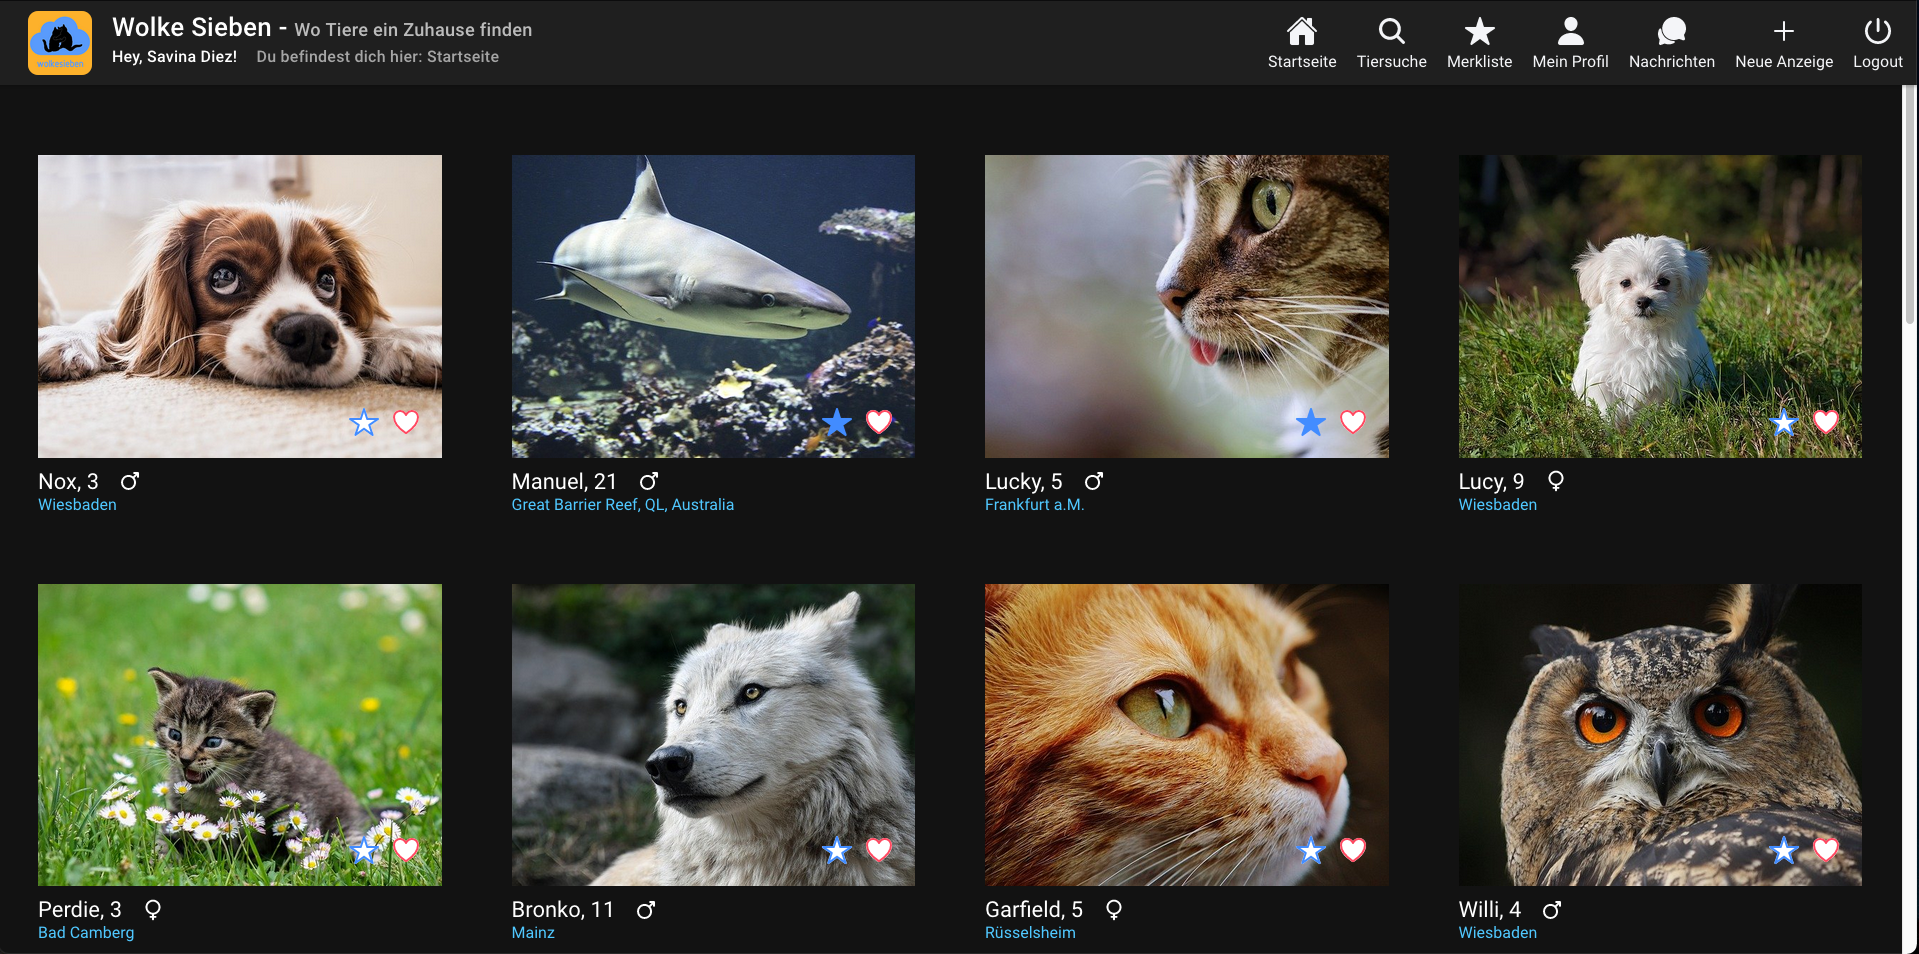
\includegraphics[width=\textwidth]{images/homepage}
\caption{Startseite von \href{https://cc-wolkesieben.de}{cc-wolkesieben.de}}
\end{figure}

Der Prototyp unserer Applikation, wie in Abbildung \ref{fig:homepage} demonstriert, ist ab sofort unter folgender Adresse aufrufbar: \url{https://cc-wolkesieben.de}.

% Why leverage cloud computing? Comparison to alternative hosting methods

\section{Architektur} % Arne
\subsection{Microservices}

Wie für Cloud-Anwendungen üblich, setzen wir bei der Struktur des Backends auf einen Microservice-Ansatz bei dem die ganzheitliche API in verschiedene, voneinander unabhängige Programme aufgeteilt wird. Diese Form der Bereitstellung hat einige Vorteile, die hier nochmal herausgestellt werden sollen.

Zum einen können die einzelnen Funktionen auf diese Weise in Umgebungen bereitgestellt werden, welche speziell auf diese zugeschnitten sind. In unserer Anwendung sieht man dies primär anhand der Aufteilung nach den verwendeten Datenbank-Typen (Polyglott Persistency). Im Umkehrschluss, muss sich jeder Microservice somit auch nur mit denen für seine Domäne relevanten Technologien befassen. Die erleichtert die Konfiguration und trägt dazu bei, dass sich Services einfacher unter den Entwicklern eines Team aufteilen lassen, ohne dass diese sich in die Quere kommen. Zu guter Letzt lassen sich die Möglichkeiten der Bereitstellung in der Cloud so optimal ausnutzen, da jeder Microservice auf der Infrastruktur aufgesetzt werden kann, die für ihn am geeignetsten ist, ohne den Rest der Anwendung auf einen Kompromiss zu forcieren. Dies wiederum erlaubt die unabhängige Skalierung der am meisten nachgefragten Teilbereiche, d.h. Microservices, der ganzheitlichen API. 

\begin{figure}[H]
\centering
\label{fig:architecture}
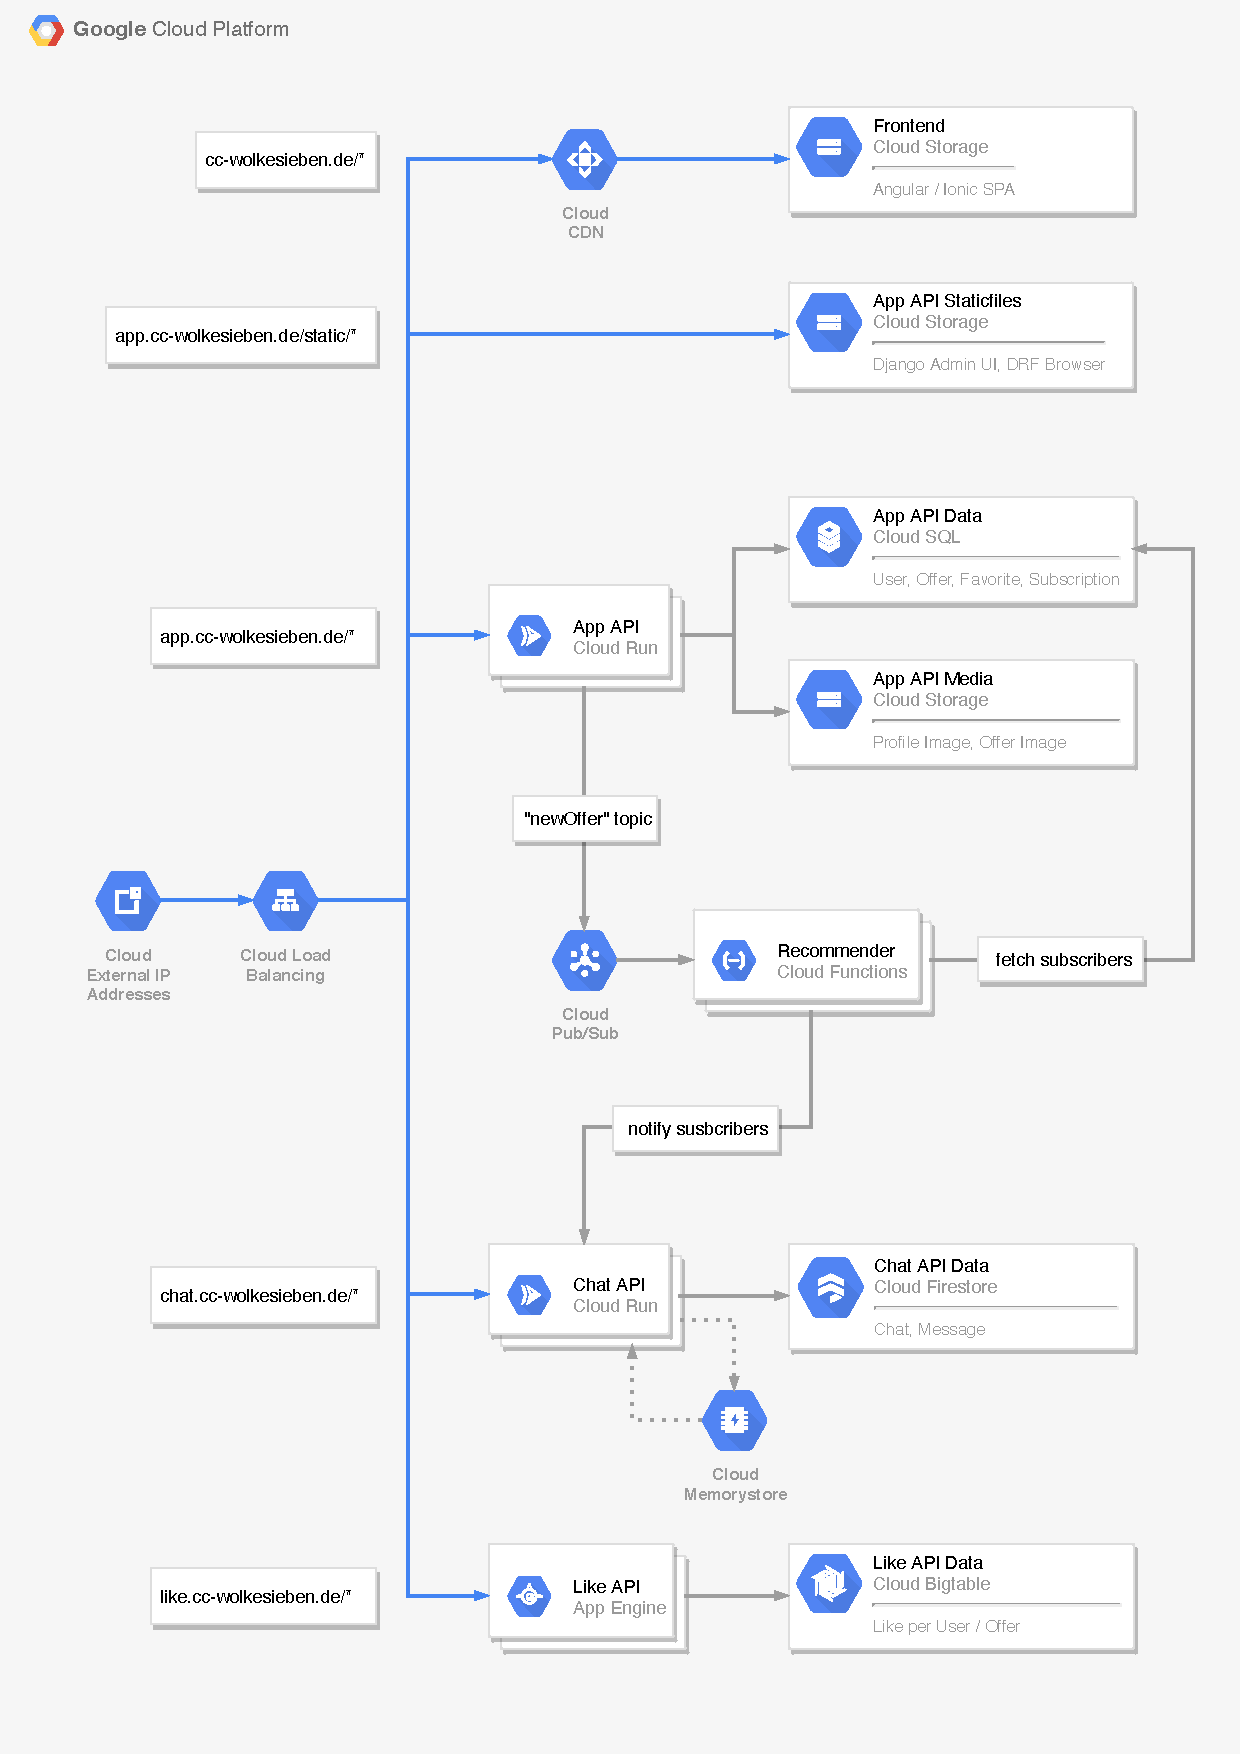
\includegraphics[width=\textwidth]{images/gcp-architecture}
\caption{Architekturüberblick}
\end{figure}

% Swagger documentation available for each service


\subsection{Domain-Driven Design}

Ursprünglich sollte sich die Architektur der einzelnen Microservices am Domain-Driven Design Pattern orientieren. Dieses sieht eine Unterteilung der Services wie folgt vor:

\begin{description}
	\item[Domäne]
	\hfill \\
	für die Kernfunktionen des Service
	\item[API]
	\hfill \\
	für die Bereitstellung
	\item[Infrastruktur]
	\hfill \\
	für die Anbindung an externe Systeme (z.B. Datenbanken)
\end{description}

\begin{figure}[htbp]
\centering
\label{fig:domaindrivendesign}
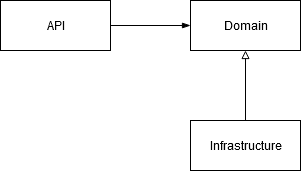
\includegraphics[width=0.5\textwidth]{images/domain-driven-design}
\caption{Domain-Driven Design}
\end{figure}

Im Laufe der Entwicklung stellte sich heraus, dass sich das Pattern, welches eigentlich für DotNet-Anwendungen konzipiert wurde, nicht so einfach auf die von uns verwendeten Programmiersprachen und Frameworks übertragen lässt. 

Konkret, soll dies am Beispiel von Django, einem Python Web-Framework, verdeutlicht werden: Einer der Hauptzwecke der Infrastruktur-Komponente ist es die Anbindung verschiedener Datenbanken, sowie den Wechsel zwischen diesen so einfach und standardisiert wie möglich zu gestalten. In Django besteht dieses Problem allerdings garnicht, da die Datenbankanbindung komplett im Hintergrund stattfindet. Bei Verwendung des Django-REST-Frameworks entfällt außerdem ein Großteil der Arbeit, die zur Erstellung einer REST-API nötig ist, da auch hier vieles im Hintergrund passiert. Des weiteren gibt Django eine relativ umfassende Dateistruktur vor, die sich nur schwer mit dem Domain-Driven Design vereinen lässt. Aus diesen Gründen haben wir uns bereits zu einem frühen Zeitpunkt der Entwicklung entschieden dieses Pattern nicht länger als Orientierung zu nehmen.


\section{Frontend} % Klaus
% Deployment target: Cloud CDN
% Comparison to other hosting methods (pro/con)
% Ionic/Angular Stack > ready for mobile
% Easy-to-use WebSocket adapter
% Google OAuth login flow
% First throw. todo: verify and rephrase


\subsection{Technologie}
\label{sec:frontend-tech}

Hinsichtlich dem Ziel unsere Plattform einer möglichst großen Masse an Benutzern zugänglich zu machen, wird das Frontend mit Ionic (Version 5) entwickelt. Obwohl augenscheinlich nur Browser Technologien zum Einsatz kommen (HTML, CSS, JavaScript), kann die mit Hilfe von Ionic entwickelte Single-Page-App anschließend auch in eine native iOS bzw. Android App konvertiert werden. Intern fußt Ionic auf dem von Google propagierten Angular Framework, welches das \enquote{Two-way Binding} Paradigma umsetzt. Es unterstützt auch die von uns bevorzugte Programmiersprache TypeScript, ein Superset von JavaScript, sowie SASS als erweiterte Stylesheet-Sprache. 

% \subsubsection{Datenstruktur in Ionic}

% In Ionic gibt es verschiedene Komponenten, die im Zusammenspiel die Anwendung komplett machen

% \subsubsection*{Page}

% Jede Ansicht einer Seite ist eine eigene Page. Die Page enthält ein HTML Template für die Ansicht, eine SCSS Datei für das Styling sowie eine TypeScript Datei für die Logik. Das HTML Template hat Zugriff auf Variablen und Funktionen der TypeScript Datei, um mit der Logik zu interagieren. Weiterhin gibt es für Jede Page Routing und Moduleinstellungen, um die Seite unter einer bestimmten URL erreichbar zu machen.

% \subsubsection*{Component}

% Eine Component ist ein Template, welches in Seiten oder anderen Components eingebunden werden kann. Somit können sich oft wiederholende Strukturen vereinheitlichen und mittels HTML Tag einbinden lassen. Components lassen sich auch Parameter übergeben, sodass diese Komponenten dynamisch verwendet werden können. Components bestehen ebenfalls aus HTML-Template, Styling und Logik. Ein Routing fehlt hier aber, sodass Components immer in Pages eingebunden werden müssen und nicht alleine stehen können.

% \subsubsection*{Service}

% Ein Service besteht nur aus dem Logikteil und kann von mehreren Pages eingebunden werden. So können Funktionen Global implementiert werden und Daten zentral verarbeitet werden.

% \subsubsection*{Pipes}

% Mit Pipes können Daten in einem HTML-Template transferiert werden, ohne eine Funktion aufrufen zu müssen. Ändern sich die zu transferierenden Daten, wird die Pipe automatisch neu angewendet.


\subsection{Authentifizierung}
\label{sec:frontend-auth}

% @TODO: authentication flow diagram
Die Authentifizierung eines Benutzers wird wie in Grafik XY durchgeführt. Im ersten Schritt wird überprüft, ob bereits eine Session vorhanden ist. Diese ist durch das Vorhandensein eines gültigen JSON Web Token (JWT), ausgestellt vom 
App-Microservice (siehe \autoref{sec:app-microservice}), gekennzeichnet. Andernfalls ist der Benutzer nicht eingeloggt. In diesem Fall, kann der Nutzer sich mit einem Social Provider (Facebook, Google, GitHub etc.) einloggen. Aktuell wird nur Google unterstützt. In jedem Fall wird jedoch eine OAuth 2.0 Anfrage an den jeweiligen Provider abgesetzt, die das Öffnen dessen Single Sign-On Fenster zur Folge hat. Bei erfolgreichem Ausweisen der Identität (normalerweise durch Benutzername und Passwort, ggf. mit OTP) liefert dieses ein sogenanntes ID Token zurück, das auch dem JWT Standard folgt. In dessen Payload findet sich neben den verifizierten Benutzer Details, wie Name oder Email Adresse, auch die in der Domäne des jeweiligen Provider eindeutige ID des Nutzers. Um den Login Vorgang abzuschließen, wird das ID Token an den App-Microservice gesendet, welches die Gültigkeit anhand der Signatur prüfen kann und dieses gegen ein neues JWT austauscht. Die Notwendigkeit für ein eigens ausgestelltes JWT wird in \autoref{sec:app-backend-auth} erläutert.

Genau genommen, handelt es sich bei der Antwort des App-Microservice um ein JWT-Paar, nämlich einem Access- und Refresh-Token. Das Access-Token wird für künftige Requests an jeden der Microservices als \texttt{Bearer} Token im \texttt{Authorization} Header mitgesendet, worauf basierend die Authentifizierung und Authorisierung in jedem Microservice stattfindet. Das Refresh-Token hingegen erlaubt es dem Frontend ein neues Access-Token zu erhalten, wenn dieses seine zeitliche Begrenzung überschritten hat. Refresh-Token sind in der Regel ein vielfaches länger gültig.

Um die Login-Session auch zwischen Neuladen der Webseite beizubehalten, werden beide Tokens im \texttt{localStorage} persistiert. Damit muss der oben beschriebene Login-Prozess erst wiederholt werden, wenn sich der Nutzer längere Zeit nicht im Portal bewegt hat und somit auch beide Tokens abgelaufen sind. Bei einem manuellen Logout werden beide Tokens zwangsläufig entfernt. 


\subsection{Google OAuth Integration}

Zur einfachen Integration mit Angular, stellt Google das \texttt{gapi} NPM Package bereit. Es verwaltet den Zustand der Authentifizierung mittels eines \texttt{GoogleUser} Objektes, das auch eine Methode exponiert (\texttt{.getAuthResponse().id\_token}), um das in \autoref{sec:frontend-auth} erwähnte ID Token abzurufen. Sollte der Benutzer nicht angemeldet sein, kann der OAuth 2.0 Prozess durch die statische Methode \texttt{gapi.auth2.init()} gestartet werden. Diese Methode sollte mit der in der Google Developer Konsole konfigurierten \texttt{CLIENT\_ID} aufgerufen werden, um sicherzustellen, dass das ID Token aus dieser Login-Session und nicht der einer anderen Applikation stammt. 


\subsection{Deployment}

Wie in \autoref{sec:frontend-tech} erläutert, besteht dieser Teil des Projekts lediglich aus einem Superset von Browser-Technologien (HTML, CSS, JavaScript). Es wird kein serverseitiger Code ausgeführt, somit ist auch kein Webserver erforderlich, um die Anwendung zu hosten. Stattdessen ist es ausreichend, das Frontend in einem öffentlichen read-only Dateisystem zu speichern. Hierfür eignet sich der Google Cloud Storage ideal. Um die Latenz noch weiter zu verringern, kann der Google Cloud CDN Service eingesetzt werden. Dies wiederum setzt einen HTTP(S) Load Balancer voraus, wie im Folgendem beschrieben. 


\subsubsection{Google Cloud Storage}

Der Google Cloud Storage ist ein Cloud Speicher, um beliebige Binary Large Objects (BLOBs) zu speichern und in sogenannten Buckets (vgl. Ordner) zu verwalten. Es gibt kein Speicherlimit, stattdessen wird die Benutzung pro belegtem Gigabyte abgerechnet. Datensicherheit, Langlebigkeit sowie Verfügbarkeit werden durch die Google SLAs garantiert.

Mit dem Programm \texttt{gsutil} stellt Google eine Kommandozeilen-Schnittstelle zur Verfügung, über die auch der Frontend Bucket dieses Projektes regelmäßig aktualisiert wird.


\subsubsection{Cloud CDN \& Load Balancer}

Das Cloud Content Delivery Network (Cloud CDN) ist ein Netzwerk von Google, welches überall auf der Welt Knotenpunkte verteilt hat und damit auf die schnelle Auslieferung von Inhalten optimiert ist. Um dieses zu nutzen, muss ein HTTP(S) Load Balancer eingerichtet werden, der Anfragen an eine Domain erhält und diese an den jeweiligen Google Cloud Storage Bucket weiterleitet. Das Cloud CDN ist dazwischengeschaltet und fungiert als unabhängiger, automatischer Cache in mehreren Regionen der Welt.

Für die Skalierung bedeutet dieses Konstrukt, dass der Bucket nicht skalieren muss, denn Anfragen entstehen lediglich während dem CDN Cache-Refill bzw. beim Upload in den Bucket selbst. Bei einer steigender Anzahl von Nutzern muss nur das Cloud CDN skalieren. Hierfür sorgt Google vorbildlich.


\section{App-Microservice} % Arne
\label{sec:app-microservice}

Der App-Microservice stellt den Großteil der Backend-Funktionen unserer Anwendung bereit. Er ist in Python geschrieben, verwendet das Django Web-Framework und wird über Cloud Run bereitgestellt.


\subsection{Technologie}

Die Programmiersprache Python ergab sich aus der Wahl des Web-Frameworks. Django bietet einige entscheidende Bausteine, welche die Entwickelung von Web-Anwendungen vereinfachen und von denen auch wir großen Gebrauch gemacht haben. 

Der vorzugsweise größte Vorteil ist die vollständige Abstraktion des Datenbankmodells durch das eingebaute Object-Relational Mapping (ORM). Dies ermöglicht das Anlegen und Verwalten einer SQL-Datenbank ohne echten SQL-Code schreiben zu müssen. Modelle und Relationen können mit Python-Code definiert werden, aus denen per Konsolen-Befehl sogenannte Migrations generiert, die anschließend von Django durch Umwandlung in SQL-Code auf die Datenbank übertragen werden. Entwickler können sich dadurch auf die reine Programmierung in Python konzentrieren. 

Bei Zuhilfenahme des Django-REST-Frameworks werden auch die Standard REST-Funktionen (\texttt{GET}, \texttt{POST}, \texttt{DELETE}, etc.) für alle eigens angelegten Datenbank Modelle vor-implementiert, wodurch sich Entwickler umso mehr auf die für die Anwendung benötigten Funktionen konzentrieren können. Dieses Plugin erleichtert auch das Testen der Anwendung, in dem es eine Web Oberfläche zur Interaktion mit der API bereitstellt. 

Daneben haben sich die eingebauten Konzepte, die Anwendung produktionsreif zu machen, schon mehrfach in der Industrie bewährt. 


\subsection{Datenbank}

Entsprechend dem Polyglott Persistency Prinzips, setzt der App Microservice auf eine Cloud SQL Instanz für relationale Daten, sowie einen Cloud Storage Bucket für Medien sonstiger Art (z.B. Fotos und Videos). Hinsichtlich dem SQL-Datenbank Typen, genügt MySQL (Version 8) unseren Anforderungen. 

An dieser Stelle sollte erwähnt werden, dass zum Zeitpunkt der Entwicklung kein offizieller Emulator für den Google Cloud Storage vorliegt. Daher wurde zum Testen der Datenbankanbindung auf eine Open-Source Lösung namens \href{https://github.com/fsouza/fake-gcs-server}{\texttt{fake-gcs-server}} zurückgegriffen. 


\subsection{Authentifizierung}
\label{sec:app-backend-auth}

Wie bereits in \autoref{sec:frontend-auth} dargelegt, 

Bei der Nutzerauthentifizierung haben wir uns dazu entschieden, selbst keine Nutzerkonten zu verwalten und so Entwicklungszeit zu sparen, die wir in die eigentliche Anwendung stecken konnten. Stattdessen authentifizieren wird unsere Nutzer über Google OAuth und JWT-Tokens. Dabei verlassen wir uns nur bei der Anmeldung auf die von Google ausgestellten Token. Der App-Microservice legt nach der Bestätigung der Identität ein eigenes JWT-Token an, welches daraufhin verwendet wird, um einen Nutzer zwischen unseren Microservices zu authentifizieren.


\subsection{Deployment}


Des Weiteren haben wir uns dazu entschieden, den App-Microservice mit Cloud Run in Docker-Containern bereitzustellen. Indem wir auf Container zurückgreifen, machen wir uns die flexible Struktur der Cloud-Umgebung zu Nutzen, in der Anwendungen ortstransparent bereitgestellt werden können. Durch die Verwendung von Containern machen wir uns von der zu Grunde liegenden Hardware unabhängig und können die Möglichkeiten der Cloud voll ausschöpfen. Weiterhin erledigt sich das Thema Skalierbarkeit so quasi von selbst, da das System auf Seiten des Anbieters in der Lage ist, jederzeit neue Container zu starten oder zu stoppen, um mit den Anforderungen des eingehenden Datenverkehrs mithalten zu können.

\section{Like- und Chat-Microservices} % Nik
% Framework: NestJS (Node.JS) > comparison to Django
% Monorepo setup with separate deployment targets
% Authentication through app microservice > should use public key cryptography in future to avoid unnecessary REST calls

\subsection{Like-Microservice}
% Deployment target: App Engine > comparison to Cloud Run
% Storage: BigTable (emulator available but not fully usable)

\subsection{Chat-Microservice}
% Deployment target: Cloud Run
% Storage: Firestore (emulator available)
% WebSocket authentication > not usable in upgrade request due to limited browser WebSocket API

\section{Recommender Cloud Function} % Savina
Wenn ein neues Angebot erstellt wird, sollen diejenigen Nutzer per Chat-Nachricht benachrichtigt werden, die die jeweilige Rasse abonniert haben. Dies erfolgt mithilfe einer Publisher/Subscriber-getriggerten Google Cloud Function.
Wir haben uns für dieses Modell entschieden, da es sich bei der Recommendation um ein nicht-zeitkritisches Feature handelt.
Um die Nachricht zu senden, wurde ein Recommendation-Bot implementiert, der den jeweiligen Benutzern per Chatnachricht die Rasse sowie den Link zum neuen Angebot schickt.
Das Publishen erfolgt durch den App Microservice. Die Recommender Function stellt anschließend einen GET-Request an den App Microservice, um die betroffenen User zu bekommen. Dann wird für jeden betroffenen User ein GET-Request an den Chat Microservice gestellt, um zu prüfen, ob bereits ein Chat zwischen dem Bot und dem User existiert. Falls nein, wird ein neuer Chat angelegt. Anschließend wird die Nachricht in diesem Chat gesendet.


% Deployment target: Cloud Functions > benefits? when is it most cost efficient (high/low traffic)?
% Concept of using a dedicated DB view (vs. implementation of REST call [time-constraints])
% Trigger via PubSub > benefit to other trigger methods?
% Explain publishing via Google PubSub client form App Microservice
% Async nature of recommendation (not time critical or required to synchronous response when creating a new offer)
% Service token authentication (B2B communication)

\section{Security} % Savina
Wir haben bei der Implementierung darauf geachtet, dass wir als Betreiber sowie die Nutzer gegen die gängigsten Angriffsmethoden geschützt sind, sodass ein Abhören, Manipulieren oder Beschädigen nicht möglich ist. Im Folgenden werden unsere Lösungskonzepte vorgestellt.

\subsection{Verschlüsselung der Kommunikation}
Eine unverschlüsselte Kommunikation der Nutzer mit einem Webserver öffnet Angriffen wie Man-in-the-Middle Attack, Cross-Site-Scripting (XSS) und Session Hijacking alle Türen. Wir nutzen ausschließlich HTTPS,
wobei Webbrowser (Client) und Server mit einem nur für sie bekannten Schlüssel arbeiten.
Somit läuft sämtliche Kommunikation verschlüsselt ab und ein Angreifer kann keine Informationen extrahieren, sofern er versuchen sollte, die Kommunikation abzuhören.

\subsection{Authentifizierung und Autorisierung}
\label{sec:authentication}
Nutzer, die unsere Applikation verwenden möchten, müssen sich als erstes mit ihrem Google-Konto anmelden. Hier macht Google Gebrauch von dem OAuth 2.0 Protokoll. Das von Google ausgestellte JWT-Token verwenden wir dazu, um eine authentifizierte Anfrage an den App Microservice zu stellen, der ein eigens erstelltes, neues JWT Token zurückgibt. Dieses Verfahren macht unsere Applikationen flexibler im Umgang mit potenziellen anderen Login-Verfahren, die in Zukunft implementiert werden könnten. Außerdem können wir unsere eigene Payload, zum Beispiel die selbst erstellte UUID des Nutzers codieren. Wir erstellen nämlich eine neue UUID, da es theoretisch möglich ist, dass eine von Google zugewiesene ID identisch mit einer ID sein kann, die eine andere Plattform ausstellt.

Sämtliche Kommunikation mit den Services erfordert das Senden des von uns erstellten Tokens im \verb|Authorization| Header.
Für zusätzliche Sicherheit stellen wir außerdem ein Refresh-Token aus, mit dem nach Ablauf der Gültigkeit des Access-Tokens (fünfzehn Minuten) über den App Service ein neues Token angefragt werden kann.
Mit einem User-JWT-Token können Anfragen an den App Microservice, den Like Microservice und den Chat Microservice geschickt werden, beispielsweise um passende Tierangebote zu finden, Angebote zu erstellen oder Profilinformationen zu ändern. Ein Nutzer ist nicht dazu autorisiert, im Namen eines anderen Nutzers oder des Recommendation Bots Nachrichten zu versenden oder ein Angebot hochzuladen. Für administratorische Zwecke existiert ein entsprechendes Service Token. Der Recommendation Bot hat ebenfalls ein eigenes Token, hauptsächlich dafür, um eine Anfrage an den App Service zu stellen, der die Abonnentenliste für eine bestimmte Rasse aus der Datenbank zurückgibt.


\subsection{Weitere Lösungen}
Unsere Applikation implementiert weitere Mechanismen zur Gewährleistung der Sicherheit.

\begin{itemize}
    \item Der Datenbankzugriff erfolgt ausschließlich vom App Microservice über Django Queries. Die Querysets von Django sind vor SQL-Injektion geschützt, da ihre Abfragen mit Hilfe von Query-Parametrisierung konstruiert werden. Der SQL-Code einer Abfrage wird getrennt von den Parametern der Abfrage definiert. Da Parameter vom Benutzer bereitgestellt werden können und daher unsicher sind, werden sie vom zugrunde liegenden Datenbanktreiber escaped.~\cite{django-security}
    \item Im App Microservice haben wir die \verb|CSRF-Middleware| manuell aktiviert, die einen Schutz gegen Request Forgeries von anderen Seiten implementiert.
    \item Da wir grundsätzlich keinen User-Input in das Dateisystem einfügen, können Directory Traversal-Angriffe in unserer Applikation nicht stattfinden.
\end{itemize}

% Use table of attack vectors and detail how a protection mechanism was implemented

\section{Scaling} % Klaus
% Load Balancer setup with serverless network endpoint groups > enables individual scaling
% Services and buckets may be deployed to multiple regions > LB decides which is the closets
% Some cloud resources must be in the same region in order to communicate > implications?
% Message broker for Chat microservice [Nik]
% Stateless REST enables horizontal scaling


\section{Continuous Integration und Continuous Delivery} % Arne + Nik
\paragraph{}
Bei Bau und Bereitstellung der verschiedenen Teile unserer Anwendung haben wir uns die Möglichkeiten der Continuous Integration sowie der Continuous Delivery (CI/CD) zu Nutze gemacht. Dies erschien uns als natürlicher Schritt, da GitHub, welches wir zur Versionsverwaltung genutzt haben, diese Konzepte selbst unterstützt. Über die sogenannten GitHub Actions kann der Code per CI/CD gebaut und bereitgestellt werden, ohne dass hierfür eine separate Plattform eingerichtet werden muss. Wir haben uns dazu entschieden, die notwendigen Dateien (Dockerfile u.ä.) im selben Projekt wie den Quellcode zu halten. Diese Entwicklungsmethode ist als "{Docker-Native}"{ }bekannt und zielt darauf ab, die Docker-Dateien an den Quellcode zu koppeln und die Verwaltung zu vereinfachen.

Für die Bereitstellung selbst haben wir das YAML-Format verwendet, mit dem sich die gewünschten Ressourcen als eine Art Skript beschreiben lassen. Dieses können die Cloud-Dienste dann für die automatische Provisionierung der Hardware benutzen.

Eine Schwierigkeit, die uns beim Bereitstellen der Microservices, die Cloud Run benutzen, aufgefallen ist, ist dass das System es offenbar nicht erlaubt, eine SSH-Sitzung in einem laufenden Container zu starten. Für die Bereitstellung ließ sich dieses Problem umgehen, da alle hierfür erforderlichen Konsolenbefehle sowieso in der YAML-Datei definiert werden müssen, um automatische ausgeführt werden zu können. Für die Wartung im laufenden Betrieb ergibt sich jedoch das Problem, dass keine Fehleranalyse stattfinden kann, da nicht auf die Fehlermeldungen zugegriffen werden kann. Hier wird eine ausgefeiltere Logging-Methode benötigt werden, um den reibungslosen Betrieb sicherzustellen. Uns ist Weiterhin bekannt, dass andere Cloud-Anbieter diese Möglichkeit sehr wohl zur Verfügung stellen. Dies wird sicherlich einen Einfluss auf die Wahl der Plattform für zukünftige Cloud-Projekte haben.

% \subsubsection{Continious Delivery, Continious Integration}

% Mit den GitHub Actions stellt GitHub eine virtuelle Maschine zur Verfügung, die es ermöglicht, Aktionen nach einem Push oder Pull Request auszuführen. Für das Frontend wird nach jedem Push ein \verb|ionic build --prod| ausgeführt und der dabei entstandene Build Ordner in den Google Cloud Bucket hochgeladen. Somit reicht ein \verb|git push|-Befehl oder ein Pull-Request aus, um ein vollständiges Deployment durchzuführen

\section{Kostenanalyse} % Klaus
% Cost per month in relation to requests / users per month

Um die Kosten für eine bestimmte Anzahl Benutzern zu berechnen, müssen zuvor einige Annahmen getroffen werden.

\subsection{Annahmen zum Nutzerverhalten}
Verglichen mit anderen Plattformen, treffen wir die Annahme, dass es im Wesentlichen zwei Nutzergruppen gibt. Eine Gruppe nutzt die Anwendung hauptsächlich zum Stöbern und Kaufen, die andere Gruppe nutzt die Anwendung zum Anbieten von Tieren. Ein kleiner Anteil der Benutzer wird sowohl kaufen als auch verkaufen. So kommen wir zu der Annahme, dass ein Benutzer im Durchschnitt zwei Inserate online hat. 

Weiterhin gehen wir davon aus, dass jedes Angebot im Durchschnitt zwei Bilder und ein Video beinhaltet, was bei einer Größe von zwei MB pro Bild und 16 MB pro Video zu einem Gesamtspeicherplatz von etwa 20 MB pro Angebot führt.

Um den Datenverkehr zu berechnen, gehen wir davon aus, dass ein registrierter Benutzer pro Tag ein Angebot aufruft sowie fünf mal die Startseite besucht. Diese Zahl haben wie etwas höher angesetzt, da auch nicht registrierte Benutzer die Startseite aufrufen können und die Anzahl dieser Aufrufe schwierig vorherzusagen sind.

Zusammengefasst haben wir folgende Parameter festgelegt:

\begin{center}\label{tab:Parameters}
\begin{tabular}{|l|l|}
    \hline
    Anzeigen pro Benutzer & 2 \\ \hline
    Speicherplatz pro Anzeige & 20 MB \\ \hline
    Datenverkehr pro Nutzer pro Monat & 600 MB \\ \hline
    Anzahl Likes pro Anzeige und Benutzer & 2 \\ \hline
    Anzahl Chats pro Benutzer pro Monat & 2 \\\hline
    Anzahl Nachrichten pro Chat & 6 \\\hline
    Größe einer Nachricht & 20 KB \\ \hline
\end{tabular}    
\end{center}

Aus den Werten der Tabelle \ref{tab:Parameters} kann man mithilfe des Google Cloud Platform-Preisrechners berechnen, welche Cloud Services welche Kosten verursachen.~\cite{google-pricing}

\begin{figure}[htbp]
\centering
\label{fig:pricingUsers}
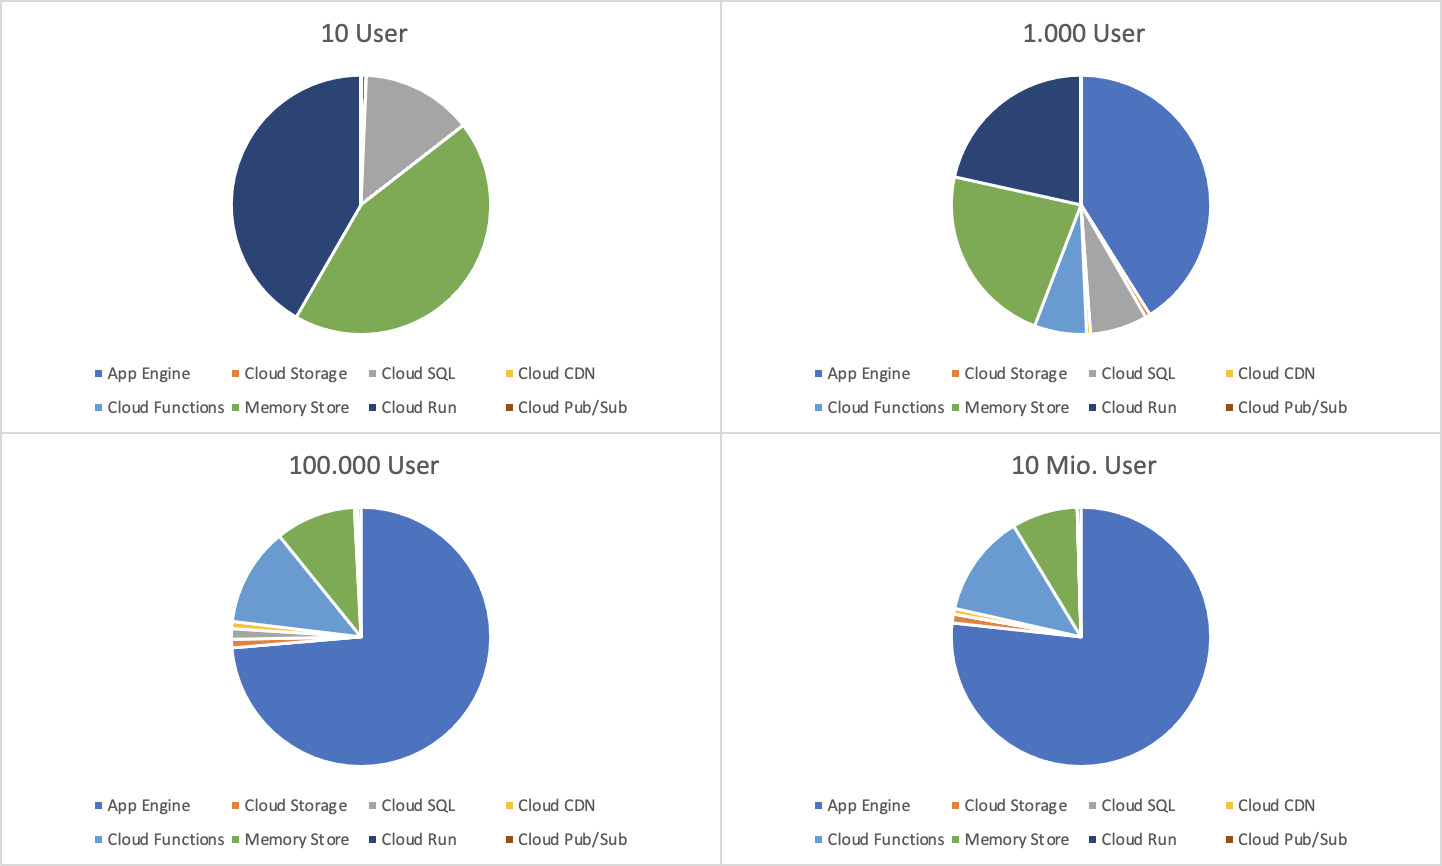
\includegraphics[width=\textwidth]{images/pricing-users}
\caption{Kostenanteil der einzelnen Services}
\end{figure}

Abbildung \ref{fig:pricingUsers} zeigt den Kostenanteil der Cloud Services im Verhältnis zu den Gesamtkosten.

\begin{figure}[htbp]
\centering
\label{fig:totalCost}
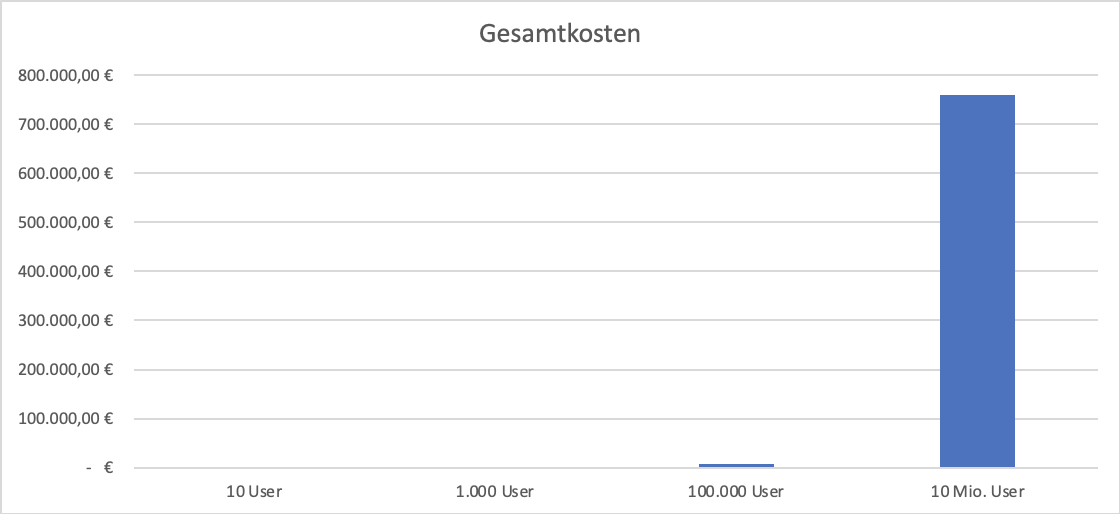
\includegraphics[width=\textwidth]{images/total-cost}
\caption{Gesamtkosten gruppiert nach Nutzerzahl}
\end{figure}

\begin{figure}[htbp]
\centering
\label{fig:costPerUser}
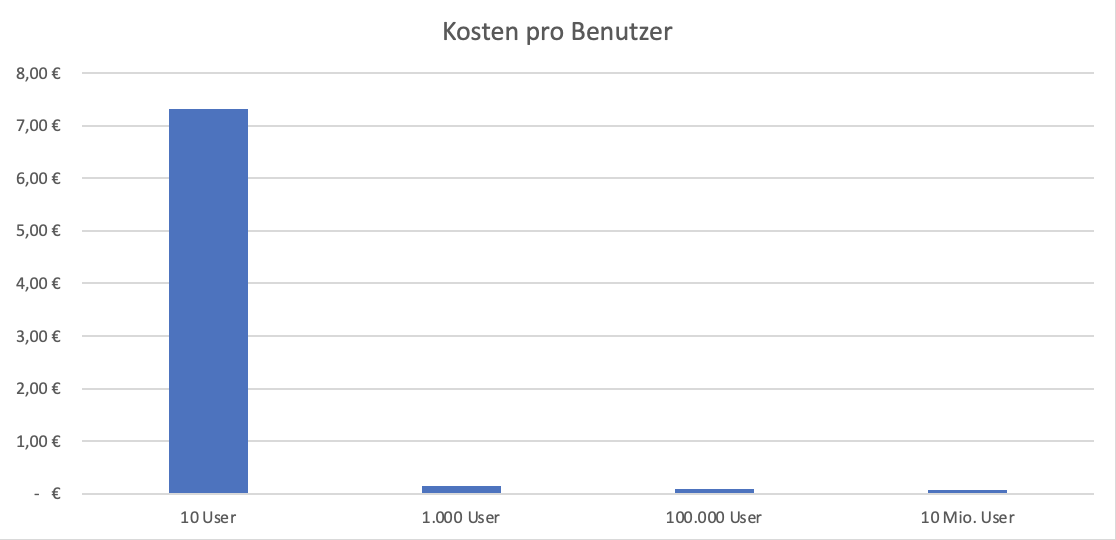
\includegraphics[width=\textwidth]{images/cost-per-user}
\caption{Gesamtkosten gruppiert nach Nutzerzahl}
\end{figure}





\appendix
% Swagger Docs (JSON export / links to production)
% Screenshots
% Larger architecture diagrams
% Individual service diagrams
% Google Cloud specific deployment diagram



\bibliography{sources.bib}{}
\bibliographystyle{plain}

\end{document}
